\section{Ejercicio 7}

En este ejercicio se pide estudiar el comportamiento del scheduler Mistery y realizar una implementación que lo imite.
Para esto se realizaron una serie de simulaciones variando primero la cantidad de parámetros y luego usando distintos lotes de tareas.

Las principales características observadas del scheduler son:
\begin{itemize}
\item La cantidad de parametros recibidos indican la cantidad de $colasReady$ que va a tener el Sched.
\item Siempre hay una cola con quantum 1, es la primera.
\item Cada parámetro es el quantum asignado a cada cola. Si los argumentos son $2 6 3$, la primera cola tendrá 2 ciclos de clock
la segunda 6 y la tercera 3.
\item El método $load(pid)$ encola a las tareas en la primera colaReady. 
\item Si una tarea termina el quantum asignado a esa cola, se le quita el cpu y se la encola en la cola siguiente. Si estaba en la ultima cola, se la encola ahí.
\item Si se le pasa un 0 como parámetro una vez que llegue una tarea a esa cola, va a ejecutarse hasta hacer EXIT.
\item Las colas tienen prioridad, y van de menor a mayor. Es decir, si una tarea esta en ejecutando en la cola $colaReady[2]$ y llega tareaNueva, se va a encolar
en $colaReady[0]$ y una vez que tarea sea desalojada, se le asignará el cpu a tareaNueva, ya que su cola tiene mayor prioridad.
\item Si una tarea se bloquea se desaloja y se encola en la $colaReady$ anterior a la que estaba cuando hizo la llamada bloqueante. Si estaba en la primera cola,
se encola en la primera de vuelta.
\end{itemize}


Se crearon 3 lotes de tareas que permitan identificar fácilmente estas características en los diagramas de Gantt.

el primer lote de tareas es:

\begin{itemize}

\item *2 TaskCPU 40
\item @20:
 *2 TaskCPU 40
\item @30:
*2 TaskCPU 30

\end{itemize}

\begin{figure}[H]
  \centering
    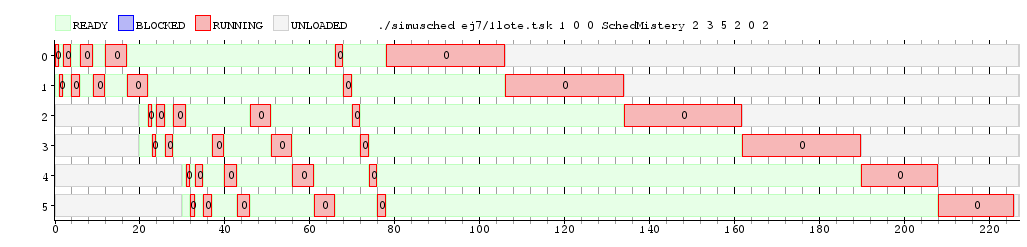
\includegraphics[width=1\textwidth]{../ej7/taskCpuMistery.png}
    \caption{Scheduler Mistery}
    %~ \label{fig:ej2_1nucleo}
\end{figure}


El costo de cambio de contexto y costa de migración de núcleo se decidió mantenerlo en 0, ya que no afecta el comportamiento del scheduler.
En el gráfico (nombre del grafico) se ve que las tareas se encolaron en la primera $colaReady$, ejecutan durante un solo tick y luego se encolan en 
la cola siguiente, que es la que tiene un quantum asociado igual a 2. El comportamiento sigue hasta que en el instante 20 llegan dos tareas nuevas.
Cuando la tarea 1 termina su quantum (instante 23), se empiezan a ejecutar las tareas en las colas con mayor prioridad, es decir 
las que acaban de llegar. Lo mismo sucede cuando llegan las tareas 4 y 5 en el el ciclo 30 de la simulación. Notar que las tareas 0 y 1 no vuelven
a obtener uso del cpu hasta el tick número 66. Esto es porque el scheduler le da prioridad a las tareas mas nuevas, ya que se encolan en las colas con
mayor prioridad. Esta característica podría hacer que las tareas mas "viejas" tarden demasiado tiempo en obtener el cpu si continuamente estan llegando 
nuaves tareas al sistema. 
Otra característica a observar es que efectivamente cuando se le asigna una tarea a la cola con quantum asociado 0, esta va a correr hasta hacer EXIT.

Para poder estudiar con mayor facilidad el comportamiento del scheduler cuando una tarea se bloquea, se creó dos tareas $Task1$ y $Task2$, que no reciben ningún
parámetro, hacen uso de cpu y realizan llamadas bloqueantes. 

El lote de tareas es:

\begin{itemize}

\item Task2BLOCK
\item Task1BLOCK
\item @15:
	TaskCPU 20

\end{itemize}

\begin{figure}[H]
  \centering
    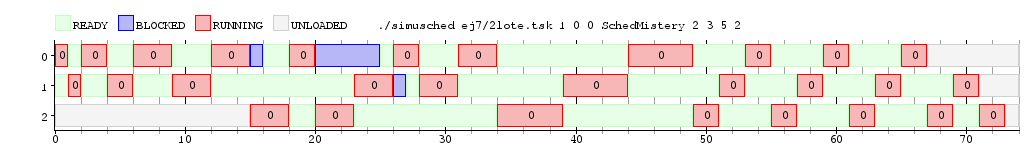
\includegraphics[width=1\textwidth]{../ej7/todojuntomistery.png}
    \caption{Scheduler Mistery}
    %~ \label{fig:ej2_1nucleo}
\end{figure}


En el instante 0 llegan dos tareas. La tarea 0 es $Task2BLOCK$ y la tarea 2 es $Task1BLOCK$. En el ciclo de clock número 15 llega la $TaskCPU$ y
las dos primeras tareas ya ejecutaron el quantum correspondiente a las tres primeras colas. En el instante 12, la tarea 0 se encuentra en la cola de con 
cantidad de quantum asociado 5. Pero en el ciclo 14 realiza una llamada bloqueante por lo que el scheduler la desaloja, y pasa a ejecutar a la tarea 2 que fue la 
última en llegar al sistema. Notar que como no hay ninguna otra tarea en las colas con quantum 1 y 2, solo la tarea 2 hace uso exclusivo del cpu 
del momento 15 al 18. Pero como al bloquearse una tarea, el scheduler la encola en la cola anterior a la que estaba, ahora pasa a ejecutar la tarea 0 nuevamente.
De nuevo realiza otra llamada bloqueante, por lo que ahora esta tarea va a pasar a la cola con quantum 2. Esto lo podemos observar en el instante 26, la tarea 0 
se ejecuta dos ciclos de clock. despues una vez que vuelve a hacer uso del cpu, realiza 3 ciclos y por ultimo pasa a la cola de quantum 5 y luego quantum 2 hasta que finaliza.
La tarea 1 también se realiza una llamada bloqueante en el tick número 25 en el momento que estaba en la cola de quantum 5. Se puede ver que la siguiente vez que 
ejecuta, se le asigna 3 ciclos de clock, que era lo esperado. 





